\documentclass[11pt,a4paper,landscape]{article}
\usepackage[margin=15mm,headheight=14pt,headsep=5mm,footskip=8mm]{geometry}
\usepackage[T1]{fontenc}
\usepackage{lmodern,microtype,xcolor,tikz,tabularx,booktabs,array,fancyhdr,hyperref}
\usetikzlibrary{arrows.meta,positioning}
\renewcommand{\familydefault}{\sfdefault}
\definecolor{navy}{HTML}{183447}
\definecolor{teal}{HTML}{147B80}
\definecolor{pale}{HTML}{EDF6F5}
\definecolor{slate}{HTML}{526574}
\definecolor{rule}{HTML}{CDDDE2}
\definecolor{sand}{HTML}{FCF3E4}
\hypersetup{colorlinks=true,urlcolor=teal,pdftitle={FININ: two-page prototype meeting brief}}
\pagestyle{fancy}\fancyhf{}
\fancyhead[L]{\small\color{slate}FININ / PROTOTYPE PROGRESS}
\fancyhead[R]{\small\color{slate}4 OCTOBER 2026}
\fancyfoot[L]{\scriptsize\color{slate}Based on Wang, Cohen \& Ma, Findings of EMNLP 2024}
\fancyfoot[R]{\small\color{slate}\thepage\ / 2}
\renewcommand{\headrulewidth}{0pt}
\setlength{\parindent}{0pt}\setlength{\parskip}{6pt}
\renewcommand{\arraystretch}{1.18}\setlength{\tabcolsep}{7pt}
\newcolumntype{Y}{>{\raggedright\arraybackslash}X}
\newcommand{\heading}[1]{{\fontsize{24}{28}\selectfont\bfseries\color{navy}#1}\par}
\newcommand{\sub}[1]{\vspace{3pt}{\large\bfseries\color{navy}#1}\par}
\newcommand{\callout}[1]{\colorbox{pale}{\parbox{\dimexpr\linewidth-2\fboxsep}{\vspace{5pt}#1\vspace{5pt}}}\par}
\tikzset{box/.style={draw=rule,rounded corners=3pt,align=center,text width=4.2cm,minimum height=1.38cm,inner sep=5pt,font=\small,text=navy},core/.style={box,fill=pale,draw=teal},arr/.style={-{Stealth[length=2mm]},line width=.8pt,draw=slate}}
\begin{document}
\heading{From the paper's idea to our prototype}
\textbf{Goal:} use financial news and market data to predict whether the next trading session closes higher.

\callout{\textbf{The key idea:} first read headlines \textbf{in relation to each other}, then use the market situation to decide \textbf{how much weight each headline receives}.}

\sub{Same core pipeline, smaller inputs}
\begin{center}
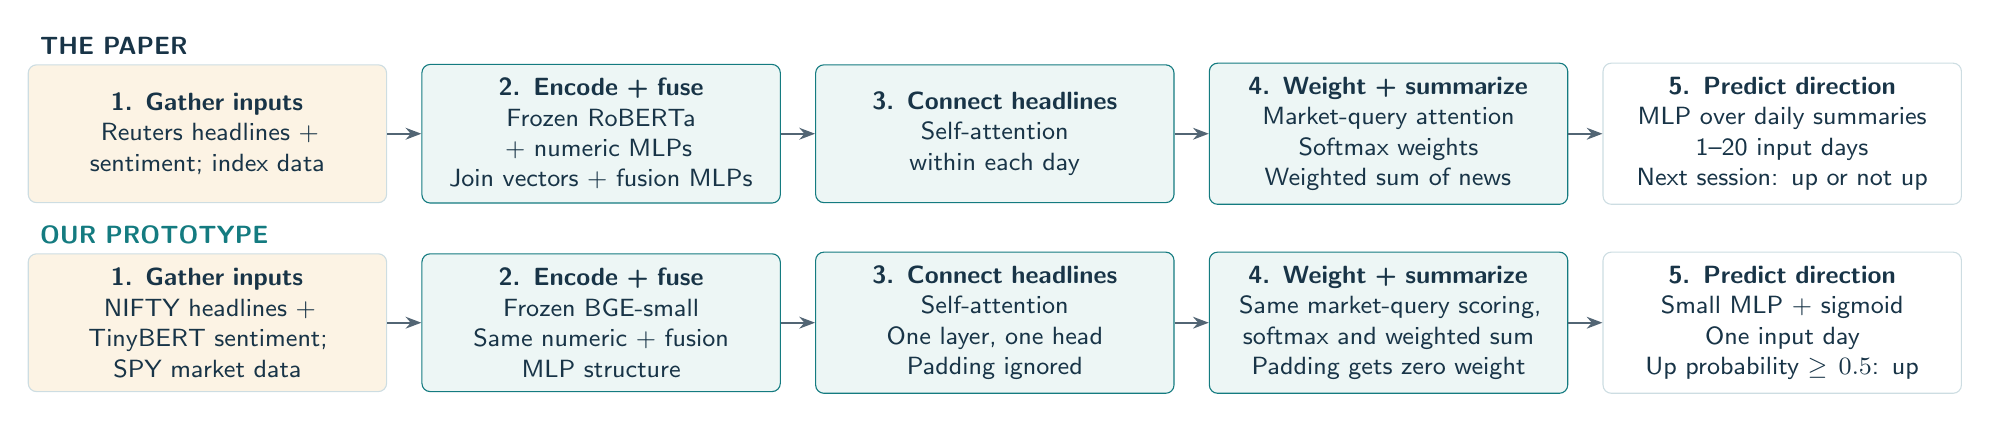
\begin{tikzpicture}[x=1cm,y=1cm]
\node[anchor=west,font=\small\bfseries,text=navy] at (-2.25,1.12) {THE PAPER};
\node[box,fill=sand,minimum height=1.75cm] (p1) at (0,0) {\textbf{1. Gather inputs}\\Reuters headlines +\\sentiment; index data};
\node[core,minimum height=1.75cm] (p2) at (5,0) {\textbf{2. Encode + fuse}\\Frozen RoBERTa\\+ numeric MLPs\\Join vectors + fusion MLPs};
\node[core,minimum height=1.75cm] (p3) at (10,0) {\textbf{3. Connect headlines}\\Self-attention\\within each day};
\node[core,minimum height=1.75cm] (p4) at (15,0) {\textbf{4. Weight + summarize}\\Market-query attention\\Softmax weights\\Weighted sum of news};
\node[box,minimum height=1.75cm] (p5) at (20,0) {\textbf{5. Predict direction}\\MLP over daily summaries\\1--20 input days\\Next session: up or not up};
\foreach \a/\b in {p1/p2,p2/p3,p3/p4,p4/p5}{\draw[arr](\a)--(\b);}
\node[anchor=west,font=\small\bfseries,text=teal] at (-2.25,-1.28) {OUR PROTOTYPE};
\node[box,fill=sand,minimum height=1.75cm] (o1) at (0,-2.4) {\textbf{1. Gather inputs}\\NIFTY headlines +\\TinyBERT sentiment;\\SPY market data};
\node[core,minimum height=1.75cm] (o2) at (5,-2.4) {\textbf{2. Encode + fuse}\\Frozen BGE-small\\Same numeric + fusion\\MLP structure};
\node[core,minimum height=1.75cm] (o3) at (10,-2.4) {\textbf{3. Connect headlines}\\Self-attention\\One layer, one head\\Padding ignored};
\node[core,minimum height=1.75cm] (o4) at (15,-2.4) {\textbf{4. Weight + summarize}\\Same market-query scoring,\\softmax and weighted sum\\Padding gets zero weight};
\node[box,minimum height=1.75cm] (o5) at (20,-2.4) {\textbf{5. Predict direction}\\Small MLP + sigmoid\\One input day\\Up probability $\geq 0.5$: up};
\foreach \a/\b in {o1/o2,o2/o3,o3/o4,o4/o5}{\draw[arr](\a)--(\b);}
\end{tikzpicture}
\end{center}
{\small\color{slate}\textbf{How the blocks work:} text shares an encoder/projection; numbers use separate MLPs. Fusion joins text and numbers for each headline and for the market. The market queries the updated news; softmax turns scores into weights, then a weighted sum creates one news summary. Market features also feed the predictor.}

\sub{The essential differences}
\begin{tabularx}{\linewidth}{@{}p{3cm}YY@{}}
\toprule
 & \textbf{Paper} & \textbf{Our prototype}\\\midrule
\textbf{Data} & S\&P 500 + NASDAQ 100; 2003--2018 & SPY (S\&P 500 ETF proxy); 2010--2020\\
\textbf{News} & Over 2.7 million Reuters items & 2,107 usable dates; at most 16 NIFTY headlines/date\\
\textbf{Text / sentiment} & RoBERTa in main results; Reuters sentiment & BGE-small text vectors; TinyBERT sentiment\\
\textbf{Experiment} & 1--20 input days; ten time windows & One input day; one time split; three training seeds\\
\bottomrule
\end{tabularx}\par
\vspace{3pt}
{\small \textbf{MLP} = a small feed-forward neural network. \textbf{Softmax} = weights that sum to one. The lookback changes; the forecast stays \textbf{one session ahead}.}

\newpage
\heading{What is working, and what have we learned?}
\sub{The prototype runs from data to saved predictions}
\begin{center}
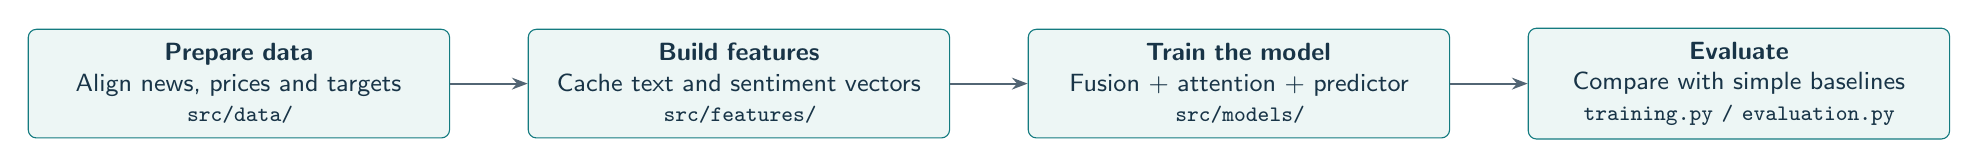
\begin{tikzpicture}
\node[core,text width=5cm] (a) at (0,0) {\textbf{Prepare data}\\Align news, prices and targets\\{\footnotesize\ttfamily src/data/}};
\node[core,text width=5cm] (b) at (6.35,0) {\textbf{Build features}\\Cache text and sentiment vectors\\{\footnotesize\ttfamily src/features/}};
\node[core,text width=5cm] (c) at (12.7,0) {\textbf{Train the model}\\Fusion + attention + predictor\\{\footnotesize\ttfamily src/models/}};
\node[core,text width=5cm] (d) at (19.05,0) {\textbf{Evaluate}\\Compare with simple baselines\\{\footnotesize\ttfamily training.py / evaluation.py}};
\draw[arr](a)--(b);\draw[arr](b)--(c);\draw[arr](c)--(d);
\end{tikzpicture}
\end{center}
{\small\color{slate}\textbf{Frozen:} pretrained BGE-small and TinyBERT. \textbf{Trained:} text projection, numeric/fusion MLPs, attention and predictor.}

\begin{minipage}[t]{.55\linewidth}
\sub{One prediction, explained simply}
\textbf{6 Jan: news} $\longrightarrow$ \textbf{7 Jan: forecast} $\longrightarrow$ \textbf{8 Jan: answer}

Use the news from 6 January and prices through the close of 7 January. Predict whether 8 January closes higher.

{\small We delay news by one trading session because individual publication times are missing. Future prices never enter the model's inputs.}
\end{minipage}\hfill
\begin{minipage}[t]{.4\linewidth}
\sub{Verified, not just implemented}
\textbf{2,107 examples} rebuilt and checked.\par
\textbf{18 training runs} reproduce saved predictions.\par
\textbf{7 integrity tests} pass.\par
{\small Data split: 1,475 train / 315 validation / 317 test.}
\end{minipage}

\sub{The result: a working prototype, with no clear forecasting gain yet}
\begin{tabularx}{\linewidth}{@{}Yrr@{}}
\toprule
\textbf{On the same 317 test dates} & \textbf{Correct predictions} & \textbf{Balanced accuracy$^*$}\\\midrule
Always predict up & 58.0\% & 50.0\%\\
Our reduced FININ & 58.4\% & 50.4\%\\
\bottomrule
\end{tabularx}\par
{\small $^*$Gives equal importance to up and non-up days. Prototype values are averages across three seeds.}

\callout{\textbf{Why the scores are close:} the model predicts up on 312--317 of the 317 dates. It mostly follows the majority class. The experiment does \textbf{not yet show that news attention improves prediction}.}

\textbf{Next step:} investigate this behavior on training/validation data, then test longer news histories against the same simple baselines using a fresh temporal evaluation.

\vfill
{\scriptsize\color{slate}\textbf{Sources:} Wang, Cohen \& Ma (2024), \href{https://aclanthology.org/2024.findings-emnlp.189/}{\emph{Modeling News Interactions and Influence for Financial Market Prediction}}, Figure 2 and Sections 3--5; \href{https://huggingface.co/datasets/raeidsaqur/NIFTY}{NIFTY dataset}; local experiments and audit. This is an architectural prototype; the paper's published gains have not been reproduced.}
\end{document}
